%%=============================================================================
%% Methodologie
%%=============================================================================

\chapter{\IfLanguageName{dutch}{Methodologie}{Methodology}}
\label{ch:methodologie}

%% TODO: Hoe ben je te werk gegaan? Verdeel je onderzoek in grote fasen, en
%% licht in elke fase toe welke stappen je gevolgd hebt. Verantwoord waarom je
%% op deze manier te werk gegaan bent. Je moet kunnen aantonen dat je de best
%% mogelijke manier toegepast hebt om een antwoord te vinden op de
%% onderzoeksvraag.



Na de stand van zaken die gebaseerd is op de literatuurstudie volgt de volgorde van stappen die ondernomen zijn om deze proef te voltooien. 

\section{z/OS Health Checker standaard setup}
\label{sec:z/OS Health Checker Standaard setup}

De eerste onderzoeksvraag was of er mogelijkheid was tot een standaardopstelling binnen de z/OS Health Checker omgeving van HCL Technologies. Maar eerst moet er een analyse plaatsvinden op de huidige opstelling van Health Checker. Om deze te optimaliseren

\subsection{Analyse van huidige z/OS Health Checker Setup}
\label{subsec:Analyse van huidige z/OS Health Checker Setup}
De opstelling die in deze proef geanalyseerd werd bevind zich binnen een parallel sysplex. En deze parallel sysplex werken we met 4 LPARS: VT1, VT2, VT3 en VT4. Elke LPAR heeft verschillende checks. Maar na de 4 LPARS te overlopen was het duidelijk dat de meeste checks op VT1 draaien. Daarom is de analyse gefocust op VT1.

De analyse is gemaakt met de check data uit SDSF deze kan je bereiken door bij het ISPF hoofdmenu volgende optie te geven 's;ck'. Dit is S voor SDSF met als volgende optie CK voor Health Checker deze ziet er zo uit.

\begin{figure}[h]
	\centering
	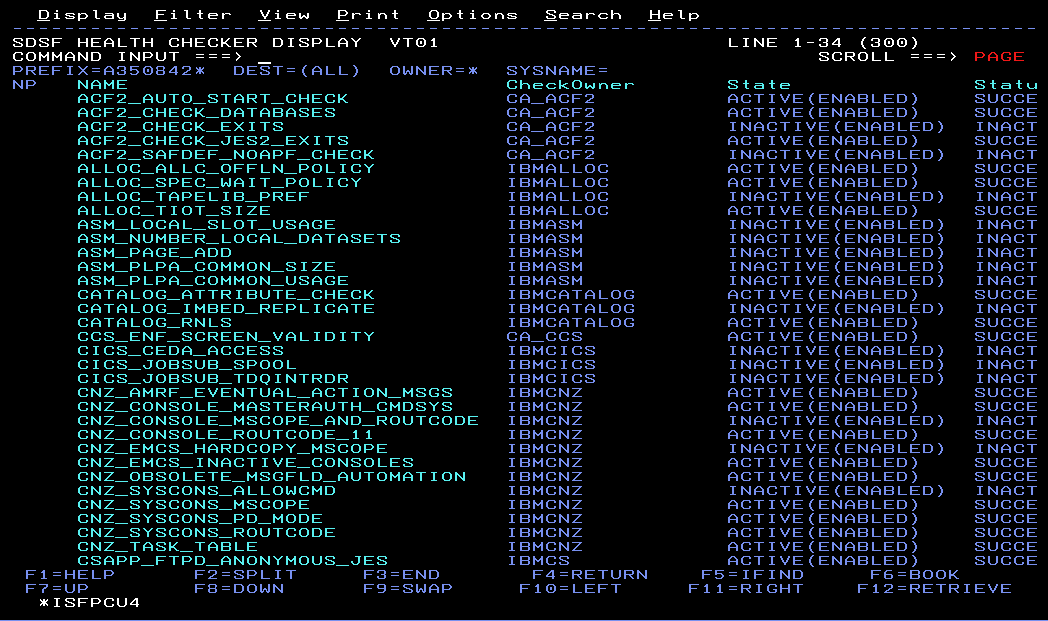
\includegraphics[width=0.7\linewidth]{img/SDSFCK}
	\caption[Health Checker Scherm binnen SDSF]{Dit is het Health Checker paneel binnen SDSF hier kunnen we de output van de laatste keren dat een check is uitgevoerd}
	\label{fig:sdsfck}
\end{figure}


Na het overlopen van alle checks op VT1 hebben we de SDSF ouptut samengevat in volgende tabel. Met de naam van de check. De status, deze beschrijft of de check aanstaat of niet. De outcome, deze beschrijft of de check succesvol was of niet. En de reason, dit is de reden waarvoor de check draait. Een voorbeeld:
\begin{table}[]
	\begin{tabular}{|p{5cm}|p{3.5cm}|p{1.5cm}|p{5cm}|}
		\hline
		\textbf{Name} & \textbf{Status} & \textbf{Outcome} & \textbf{Reason} \\
		\hline
		XCF\_CDS\_MAXSYSTEM & ACTIVE(ENABLED) & SUCCES & CDS MAXSYSTEM value across all CDS types should be at least equal to the value 
		in the primary sysplex CDS.  \\
		\hline
	\end{tabular}
	\caption[Individuele check]{Waarden van de check die bij de eerste analyse werden samengevat}
	\label{tbl:Individuele check}
\end{table}


Voor de volledige tabel zie bijlage 

Hier uit bleek dat er verscheidene check een exception hadden. Deze zijn eerst gecontroleerd of dat men deze zelf kon oplossen zonder ondersteuning van de collega's die het product beheren. Bij deze analyse bleek ook dat er veel checks zijn die onnodig draaiden omdat het product van de check bijvoorbeeld niet aanwezig was. Niet alle checks moeten in alle LPARs draaien en sommige moesten aangepast worden. Maar daarvoor heb je nog de belangrijke vraag of een wijziging van een check doorgevoerd moet worden naar alle LPARs of maar naar 1 LPAR binnen de Parallel Sysplex. Met deze informatie is naar feedback gevraagd van alle Mainframe Teams binnen HCL Technologies. Want men kan checks niet aanpassen van bijvoorbeeld DB2 zonder feedback van het DB team. Hiervoor zijn alle checks gegroepeerd per owner daarna nog eens gegroepeerd per mainframe team en uiteindelijk werd tabel \ref{tbl:Checks Per Team} bereikt.

Nog een kleine verduidelijking per team
\begin{itemize}
	\item CICS: Dit team is verantwoordelijk voor de IBM CICS Software\footnote{Customer Information Control System dit is software voor het verwerken van transacties (\cite{ChrisRayns2011}) }
	\item Communication: Dit team is verantwoordelijk voor alle communicatie-gerelateerd software zoals TCP/IP, FTP\footnote{File Transfer Protocol}, etc.
	\item Print: Dit team is verantwoordelijk voor alle output software zoals CA-View\footnote{Tool van Computer Associates}, VPS, etc.
	\item Automation: Dit team is verantwoordelijk voor alles wat met automatisering te maken heeft. Vooral software zoals System Automation, NetView en GDPS. Dit team is het meest betrokken bij monitoring.
	\item ROO: Roll-Out \& Operate, dit team beheert de 'basics' van z/OS. Dit team voert ook de upgrades uit.
	\item RTC: RunTime Control, dit team is verantwoordelijk voor performance en rapportering.
	\item Security: Dit team spreekt voor zich het beheert toels zoals RACF/ACF2/Top Secret dit zijn allemaal tool die extra beveiliging aanbieden voor de mainframe.	
	\item SOE: Standard Operating Environment, dit team doet alle installaties van software voor de mainframe.
	\item Storage: Dit team beheert alles wat te maken heeft met opslag en ook de software die erbij hoort.
	\item zOPEN: Dit team beheert alles van zLinux\footnote{Een linux besturingsysteem voor mainframe} samen met Unix System Services\footnote{UNIX besturingssysteem implementatie voor de mainframe} en Websphere\footnote{Software product gericht op web-technologie}
	\item DB: Database team, beheert alles database systemen waaronder DB2.
\end{itemize}

\begin{table}[h]
	\begin{tabular}{|l|p{9cm}|}
		\hline
		\textbf{Team}                      & \textbf{Checks(Owner)}                                                                                                                                                 \\ \hline
		\textbf{Cics}                      & IBMCICS                                                                                                                                                                \\ \hline
		\textbf{Communication}             & IBMCS, CA\_TPX                                                                                                                                                         \\ \hline
		\textbf{Print}                     & CA\_DLVR, CA\_SPOOL, CA\_VIEW                                                                                                                                          \\ \hline
		\textbf{Rollout and Opperate(ROO)} & CA\_CSS, IBMCNZ,  IMBCTRACE, IBMDAE, IBMISPF, IBMXLOGR, IBMJES(2), IBMRRS, IBMRTM, IBMSDSF, IBMSDUMP, IBMSLIP, IBMSVA, IBMSYSTRACE, IBMTIMER, IBMTSOE,  IBMXCF, IBMGRS \\ \hline
		\textbf{Run Time Control(RTC)}     & IBMVLF, CA\_PMO, IBMRCF, IBMASM, IBMRSM, IBMSUP, IBMVSM,  CPWR\_THRUPUT\_MGR                                                                                           \\ \hline
		\textbf{Security}                  & CA\_ACF2, IBMICSF                                                                                                                                                      \\ \hline
		\textbf{SOE}                       & All checks starting with ZOSMIG                                                                                                                                        \\ \hline
		\textbf{Storage}                   & CA\_DISK, IBMALLOC, IBMCATALOG, IBMDMO, IBMHSM, IMBIOS, IBMOCE, IMBPDSE, IBMSMS, IBMVSAM(RLS), CA\_VANTAGE                                                             \\ \hline
		\textbf{zOpen}                     & IBMSSH, IBMUSS, IBMZFS                                                                                                                                                 \\ \hline
		\textbf{Databse(DB)}               & CA\_DB2, CA\_DTCM, CA\_IDMS                                                                                                                                            \\ \hline
		\textbf{Automation}                & IBMGDPS                                                                                                                                                                \\ \hline
	\end{tabular}
	\caption[Checks Per team]{Alle checkowners gegroepeerd per team binnen HCL}
	\label{tbl:Checks Per Team}
\end{table}

Nadat alle checks per team werden gegroepeerd, is er eerst zelf een voorstel gemaakt voor de opstelling van hun checks waar zij feedback op konden geven. Wanneer er geen feedback was is de voorgestelde opstelling geimplementeerd.